\chapter{Introduction to the RGB-D Visual Odometry Problem}%
\label{cha:rgbd_vo}

\minitoc%
\clearpage

\section{Modeling Image Capture in a Camera}%
\label{sec:image-formation}

\subsection{Historic Remarks}%
\label{sub:historic_remarks}

The study of the image formation process has a long history.
Traces of geometric formulations of image formation are present
in Euclid work (4th century B.C.) and partially correct perspective
projections are visible in frescoes of Pompeii (1 B.C.).
These skills also re-emerged in Renaissance art with artists such as
Brunelleschi, Donatello and Alberti.
A treatise on the projection process, \textit{``Della Pittura''},
was published by Leon Battista Alberti in 1435 and influenced
many Renaissance artists such as Leonardo da Vinci and Raphael.
In Figure~\ref{fig:raphael_school_athens}
the perspective emerges from the vanishing point.
D\"urer devised a machine to get a perspectively correct image,
represented in Figure~\ref{fig:durer_perspective_machine}.
It is a manual reproduction of what a camera does today.

\begin{figure}[h]
\centering
\begin{subfigure}[b]{0.48\textwidth}
	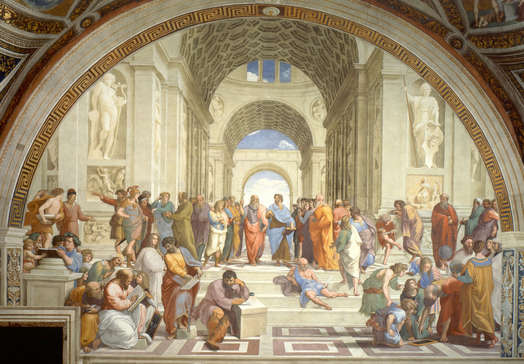
\includegraphics[width=\textwidth]{assets/img/raphael_school_athens.jpg}
	\caption{Raphael, The School of Athens (1509)}%
	\label{fig:raphael_school_athens}
\end{subfigure}
\hfill
\begin{subfigure}[b]{0.46\textwidth}
	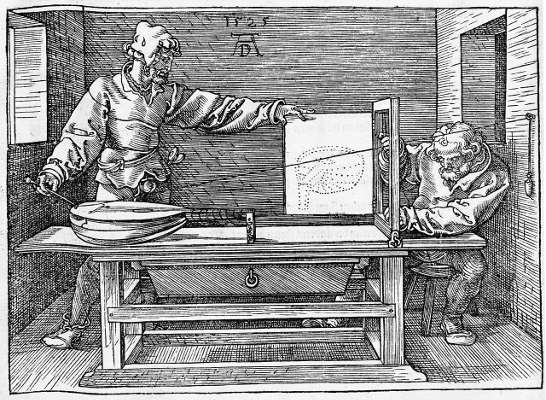
\includegraphics[width=\textwidth]{assets/img/durer_perspective_machine.jpg}
	\caption{D\"urer's perspective machine (1525)}%
	\label{fig:durer_perspective_machine}
\end{subfigure}
\caption{Usage of perspective projection in Renaissance art.}%
\end{figure}

Many artists also played with those perspective rules to create images
that seem locally correct but have inconsitent global depth or gravity
such as Hogarth (Figure~\ref{fig:hogarth_satire})
and Escher (Figure~\ref{fig:escher_belvedere}).

\begin{figure}[h]
\centering
\begin{subfigure}[b]{0.52\textwidth}
	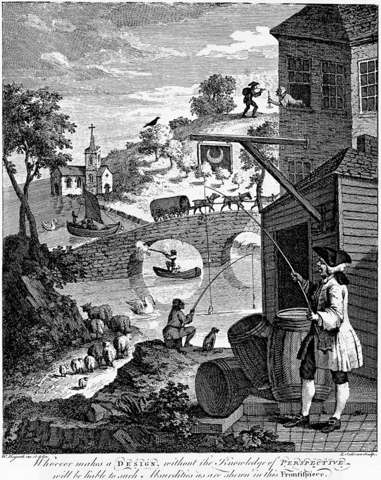
\includegraphics[width=\textwidth]{assets/img/hogarth_satire.jpg}
	\caption{Satire by Hogarth 1753}%
	\label{fig:hogarth_satire}
\end{subfigure}
\hfill
\begin{subfigure}[b]{0.42\textwidth}
	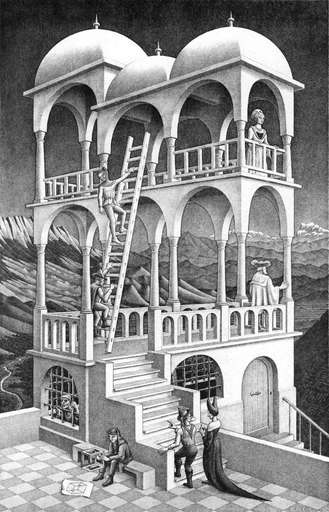
\includegraphics[width=\textwidth]{assets/img/escher_belvedere.jpg}
	\caption{Escher, Belvedere 1958}%
	\label{fig:escher_belvedere}
\end{subfigure}
\caption{Conscious circumvention of perspective projection in art.}%
\end{figure}


\subsection{Projective Geometry}%
\label{sub:projective_geometry}


In order to formally write transformations by linear operations,
we make extensive use of homogeneous coordinates to represent
3D point as a 4D-vector $(X,Y,Z,1)$ with the last coordinate fixed to 1.
This normalization is not always necessary. One can represent 3D points
by a general 4D vector
\[
	\bm{X} = (XW, YW, ZW, W)\ \in\ \R^4.
\]
In general, an n-dimensional projective space $\mathbb{P}^n$
is the set of all one-dimensional subspaces (i.e.\ lines through the origin)
of the vector space $\R^{n+1}$.
A point $p \in \mathbb{P}^n$ can then be assigned homogeneous coordinates
$\bm{X} = \tr{(x_1, \ldots, x_{n+1})}$, among which at least one $x$ is nonzero.
For any nonzero $\lambda \in \R$, the coordinates
$\bm{Y} = \tr{(\lambda x_1, \ldots, \lambda x_{n+1})}$
represent the same point $p$.


\subsection{Pinhole Camera Model}%
\label{sub:pinhole}


\begin{figure}[h]
\centering
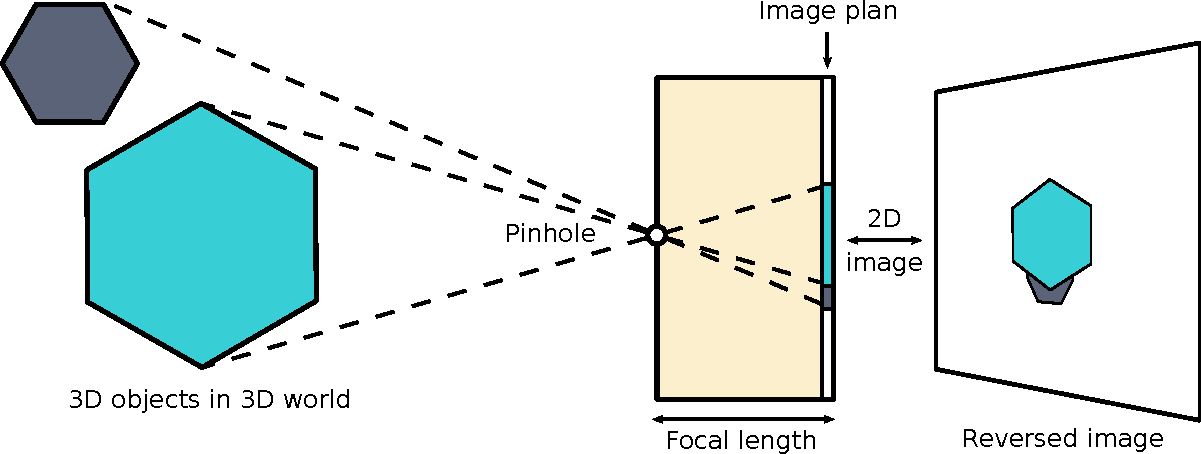
\includegraphics[width=\textwidth]{assets/img/pinhole.pdf}
\caption{Pinhole camera model.}%
\label{fig:pinhole_camera}
\end{figure}

Perspective projection emerges from a simplified model
of a real camera called the pinhole camera,
represented in Figure~\ref{fig:pinhole_camera}.
The main issue of such a camera,
is that the hole has to be very small to get a sharp image,
preventing light to enter the capture device.
In order to augment the amount of light, today we use lenses,
but just as with a pinhole camera, the image is upside down in the image plan.
In order to avoid dealing with minus signs in the equations,
we pretend that the image plan is virtually on the same side than the object.
The perspective transformation $\pi$ modeling this projection is given by
\[ \pi : \R^3 \rightarrow \R^2; \quad
	\bm{X} \mapsto x = \pi(\bm{X}) =
	\begin{pmatrix}
		f \frac{X}{Z} \\
		f \frac{Y}{Z} \\
	\end{pmatrix}
\]
where $f$ is the focal length, $X,Y,Z$ are the object coordinates
in the 3D world, the $z$ axis being the camera axis.
The one challenge we have to overcome, is that this transformation is non linear.
In order to do so, we use homogeneous coordinates,
which is basically similar to multiplying everything by $Z$,
\[ Z \bm{x} = Z \begin{pmatrix} x \\ y \\ 1 \end{pmatrix} =
	\begin{pmatrix}
		f & 0 & 0 & 0 \\
		0 & f & 0 & 0 \\
		0 & 0 & 1 & 0 \\
	\end{pmatrix}
	\begin{pmatrix}
		X \\ Y \\ Z \\ 1
	\end{pmatrix}
	= K_f \Pi_0 \bm{X}
\]
where we have introduced the two matrices
\[K_f =
	\begin{pmatrix}
		f & 0 & 0 \\
		0 & f & 0 \\
		0 & 0 & 1 \\
	\end{pmatrix}
	\quad \text{and} \quad
	\Pi_0 =
	\begin{pmatrix}
		1 & 0 & 0 & 0 \\
		0 & 1 & 0 & 0 \\
		0 & 0 & 1 & 0 \\
	\end{pmatrix}.
\]
The matrix $\Pi_0$ is referred to as the standard projection matrix.
We often note the distance to the camera along its axis with $\lambda > 0$ so
\[
	\lambda \bm{x} = K_f \Pi_0 \bm{X}.
\]


\subsection{Intrinsic Parameters}%
\label{sub:intrinsic_parameters}


If the camera is not centered at the optical center, we have an additional
translation $o_x, o_y$. The point where the optical axis intersects
the image plan is called the principal point.
If pixels do not have unit scale, we need to introduce
additional scaling factors $s_x$ and $s_y$.
And if pixels are not rectangular, we also have a skew factor $s_{\theta}$.
The transformation from coordinates in the frame of the camera
to final pixel coordinates has thus the following steps
\[
	\text{Camera}\ (\text{3D}, \bm{X})
		\quad \overset{K_f\Pi_0}{\longrightarrow} \quad
			\text{Image}\ (\text{2D}, \bm{x})
		\quad \overset{K_s}{\longrightarrow} \quad
			\text{Pixel}\ (\text{2D}, \bm{x'}).
\]
where the pixel coordinates $\bm{x'} = (x',y',1)$ are given by
$\lambda\ \bm{x'} = K_s\ K_f\ \Pi_0\ \bm{X}$
with
\[K_s = \begin{pmatrix}
		s_x & s_{\theta} & o_x \\
		0 & s_y & o_y \\
		0 & 0 & 1 \\
	\end{pmatrix}
	\quad \text{and} \quad K_f =
	\begin{pmatrix}
		f & 0 & 0 \\
		0 & f & 0 \\
		0 & 0 & 1 \\
	\end{pmatrix}.
\]
We call $K = K_s\ K_f$ the intrinsic matrix since it holds
parameters intrinsic to the camera system, independent from
the outside 3D world.


\subsection{Radial Distortion}%
\label{sub:radial_distortion}

The intrinsic parameters in the matrix $K$ model linear distortions
in the transformation to pixel coordinates.
In practice however, one can also encounter significant
distortions along the radial axis.
This is particularly visible in a wide field of view
or if one uses cheaper cameras such as webcams.
A simple effective model for such distortions is to use
\[
	x = x_d ( 1 + a_1 r^2 + a_2 r^4 ),\quad
	y = y_d ( 1 + a_1 r^2 + a_2 r^4 )
\]
where $\bm{x} = (x_d, y_d)$ is the distorted point,
and $r^2 = \|\bm{x}\|^2$ is its squared distance to the principal point.
Usually, $a_1$ and $a_2$ are estimated through a calibration step computed from
distortions of straight lines as in Figure~\ref{fig:radial_distortion}
or simultaneously with a 3D reconstruction~\cite{stein1997lens, fitzgibbon2001simultaneous}.
Other more sophisticated models exist~\cite{devernay1995automatic}
but we will not enter in details here since we will consider
that images are rectified as if fitting the pinhole model.

\begin{figure}[h]
\centering
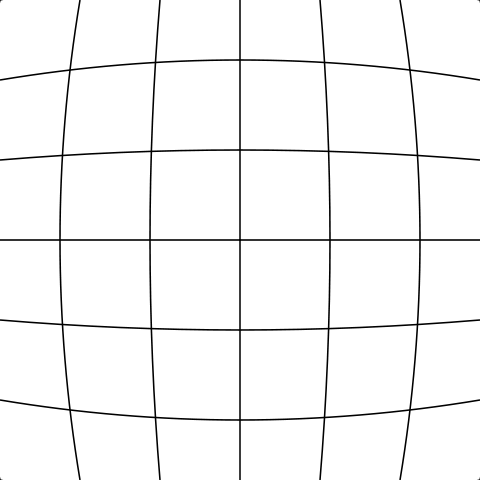
\includegraphics[width=0.5\columnwidth]{assets/img/barrel_distortion.png}
\caption{Grid projection with radial distortion.}%
\label{fig:radial_distortion}
\end{figure}


\section{Modeling Camera Movements}%
\label{sec:moving-scene}

\subsection{Origins of 3D Reconstruction}%
\label{sub:origins_of_3d_reconstruction}

Aiming to reconstruct a three-dimensional structure of the world from
a set of two-dimensional views has a long history in computer vision.
It is generally considered and ill-posed problem since reconstructions
consistent with a given set of observations/images are typically not unique.
Therefore, one need to impose additional assumptions.
The study of geometric relations between a 3D scene
and observed 2D projections is based on two types of mathematic transformations, namely
\begin{itemize}
	\item Perspective projection, and projective geometry to account for the image formation
		process we presented in the previous section.
	\item Euclidean motion or ``rigid body motion''
		representing the motion of the camera from one frame to the next.
\end{itemize}

The first known work on the problem of multiple view geometry was that of
Erwin Kruppa (1913) who showed that two views of five points
are sufficient to determine both the relative tansformation
(``motion'') between the two views and the 3D location (``structure'')
of the points up to a finite number of solutions.
A linear algorithm to recover structure and motion from two views based
on the epipolar constraint was proposed by Longuet-Higgins in 1981~\cite{longuet1981computer}.
Several summarizing text books and papers were also written
on the subject~\cite{faugeras1993three, weng1993optimal}.
Extensions to three views~\cite{spetsakis1987closed, shashua1994trilinearity}
and factorization techniques for multiple views and orthogonal projection were
also developed~\cite{tomasi1992shape}.
Depending on communities and context,
the joint estimation of camera motion and surrounding 3D environment is called
structure and motion or visual SLAM (simultaneous location and mapping).
Visual SLAM techniques slightly differ from structure and motion in the sense
that they are specialized for timely coherent sequences of images such as videos.
Visual odometry, that we will detail later, is the core step of Visual SLAM,
consisting of evaluating the camera motion of the next frame in the sequence.
Structure and motion however usually refers to situations where no such assumption
is done regarding the set of images.

\subsection{3D Space \& Rigid Body Motion}%
\label{sub:3d_space_rigid_body_motion}

\subsubsection{Three-dimensional Euclidean Space}%
\label{ssub:three_dimensional_euclidean_space}

The three-dimensional Euclidean space $\E^3$ consists of all points
$p \in \E^3$ characterized by coordinates
$\bm{X} = \tr{(X_1, X_2, X_3)} \in \R^3$
such that $\E^3$ can be identified with $\R^3$.
By identifying $\E^3$ and $\R^3$,
one can endow $\E^3$ with a scalar product, a norm and a metric.
This allows to compute distances, curve lengths, areas and volumes.


\subsubsection{Cross Product \& Skew-symmetric Matrices}%
\label{ssub:cross_product_and_skew_symmetric_matrices}

The cross product of two vectors $\bm{u}$ and $\bm{v}$ in $\R^3$ is a vector orthogonal to both.
\[
	\times : \R^3 \times \R^3 \rightarrow \R^3,\quad \bm{u} \times \bm{v} =
	\begin{pmatrix}
		u_2v_3 - u_3v_2 \\
		u_3v_1 - u_1v_3 \\
		u_1v_2 - u_2v_1
	\end{pmatrix} \in \R^3.
\]
Since $\bm{u} \times \bm{v} = -\bm{v} \times \bm{u}$, the cross product
also introduces an orientation.
Fixing $\bm{u}$ induces a linear mapping $\bm{v} \mapsto \bm{u} \times \bm{v}$
wich can be represented by the skew-symmetric matrix
\[
	\twist{u} = \cross{u} = \hatmat{u_1}{u_2}{u_3} \in \RR{3}{3}.
\]
such that $\bm{u} \times \bm{v} = \twist{u} \ \bm{v}$.
In turn, every skew symmetric matrix $M \in \RR{3}{3}$
verifying $M = -\tr{M}$
can be identified by a vector $\bm{u} \in \R^3$.
The operator $\wedge$ (``hat'') defines an isomorphism between $\R^3$
and the space $\sooo$ of the $3 \times 3$ skew-symmetric matrices.
Since a similar property is true for twists that we introduce later,
we will use the notation $\cross{u}$ instead of $\twist{u}$,
which is a visual reminder that it acts like a cross product.
Its inverse is denoted by (``vee'') $\vee : \sooo \rightarrow \R^3$.


\subsubsection{Rigid-Body Motion}%
\label{ssub:rigid_body_motion}

A rigid-body motion (or rigid-body transformation)
is a family of maps preserving the norm and cross product of any two vectors.
\begin{gather*}
	g : \R^3 \rightarrow \R^3,\quad \bm{u} \mapsto g(\bm{u}), \\
	\forall \bm{u} \in \R^3, \quad \|g(\bm{u})\| = \|\bm{u}\|, \\
	\forall\ \bm{u},\bm{v} \in \R^3, \quad g(\bm{u}) \times g(\bm{v}) =
		g(\bm{u} \times \bm{v})
\end{gather*}
Since norm and scalar product are related by the polarization identity
one can also state that a rigid-body motion is a map which
preserves inner product and cross product.
As a consequence, rigid-body motions also preserve the triple product,
and therefore volumes.
\[
	\forall\ \bm{u}, \bm{v}, \bm{w} \in \R^3, \quad
	\inner{g(\bm{u})}{g(\bm{v}) \times g(\bm{w})} =
		\inner{\bm{u}}{\bm{v} \times \bm{w}}.
\]

Let $\bm{e_1}, \bm{e_2}, \bm{e_3} \in \R^3$
be the orthonormal oriented vectors of our initial frame.
We note the transformed vectors $\bm{r_i} = g(\bm{e_i})$
and $R$ the matrix $R = (\bm{r_1}, \bm{r_2}, \bm{r_3})$
The first constraint (preservation of scalar product) implies that
$R$ is an orthogonal matrix $\tr{R}R=R\tr{R}=I$.
The second property (preservation of cross product) implies that $\det(R) = +1$.
In other words, $R$ is an element of the group
$SO(3) = \Set{R \in \RR{3}{3}} {\tr{R}R=I,\ \det(R) = +1}$.
The motion of the origin can be represented by a translation $\bm{T} \in R^3$.
Thus the rigid-body motion $g$ can be written as
\[
	g(\bm{x}) = R\bm{x} + \bm{T},\quad R \in SO(3),\quad \bm{T} \in \R^3.
\]

\subsubsection{Image Formation with Camera Movement}%
\label{ssub:projectionWithMovement}

Let's consider $\bm{X_0}$ a point in the World reference frame.
Its coordinates in the camera frame are determined by a rigid body motion
$\bm{X} = g(\bm{X_0}) = R \bm{X_0} + \bm{T}$.
In homogeneous coordinates, we can write
$\bm{X} = g\bm{X_0} = \inmatrix{ R & \bm{T}\\ 0 & 1} \bm{X_0}$.
In~\ref{sub:intrinsic_parameters}, we identified that pixels coordinates
are linked to point coordinates in the camera frame by
$\lambda\ \bm{x'} = K_s\ K_f\ \Pi_0\ \bm{X}$.
In total, the transformation from World coordinates to pixels coordinates
is given in homogeneous coordinates by
\[\boxed{
	\lambda\ \bm{x'} = K\ \Pi_0\ g\ \bm{X_0}
}\]
where $\lambda$ is the depth of the point in the camera frame,
$K$ is the intrinsics matrix, $\Pi_0$ the standard projection matrix
and $g$ the rigid body motion characterizing the camera,
also sometimes called extrinsics matrix.


\subsection{The Lie Group $SO(3)$ and Lie Algebra $\sooo$}%
\label{sub:the_lie_group_so_3}


\subsubsection{Sophus Lie (1841--1899)}%
\label{ssub:sophus_lie_1841_1899}

\begin{figure}[ht]
\centering
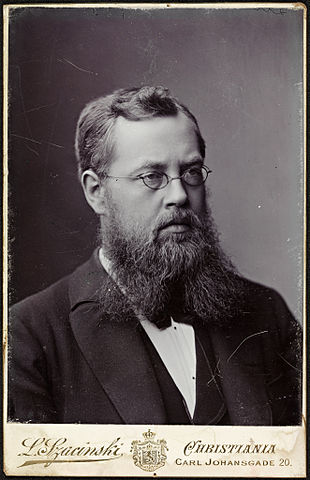
\includegraphics[width=10em]{assets/img/sophus_lie.jpg}
\caption*{Portrait of Marius Sophus Lie}
\end{figure}

Marius Sophus Lie was a Norwegian-born mathematician.
He created the theory of continuous symmetry, and applied it to
the study of geometry and differential equations.
He discovered that continuous transformation
groups are better understood in their linearized versions
(Theory of transformation groups, 1893).
These infinitesimal generators form a structure which is today
known as a Lie algebra.


\subsubsection{Lie Algebra $\sooo$}%
\label{ssub:lie_algebra_so3}

One can show that the effect of any infinitesimal
rotation $R \in SO(3)$ can be approximated by an element from
the space of skew-symmetric matrices
$\sooo = \Set{\cross{w}}{\bm{w} \in \R^3}$.
The rotation group $SO(3)$ is called a Lie group.
The space $\sooo$ is called its Lie algebra.


\subsubsection{The Exponential Map}%
\label{ssub:the_exponential_map}

Given the infinitesimal formulation of a rotation,
obtained from a continuous set of rotations $R(t)$
and by deriving the equation $R(t)\tr{R(t)} = I$,
one can show that $\dot{R}\tr{R}$ is a skew-symmetric matrix
and that we have the differential equation system
\[\left\{
	\begin{aligned}
		\dot{R}(t) &= \cross{w}(t)R(t), \\
		R(0) &= I. \\
	\end{aligned}
\right.\]
If we assume that $\cross{w}(t)$ is constant in time ($=\cross{w}$),
this known equation has the solution
\[
	R(t) = e^{\cross{w}t}
		= \sum_{n=0}^{\infty} \frac{{(\cross{w}t)}^n }{n!}
		= I + \cross{w}t + \frac{{(\cross{w}t)}^2 }{2!} + \ldots
\]
which is a rotation around the axis $\bm{w} \in \R^3$
by an angle of t (if $\|\bm{w}\| = 1$).
One can also absorb the scalar $t \in \R$ into the skew-symmetric matrix $\cross{w}$.
This matrix exponential therefore defines a map from
the Lie algebra to the Lie group
\[
	\exp : \sooo \rightarrow SO(3), \quad \cross{w}\mapsto e^{\cross{w}}.
\]
In analogy to the well-known Euler equation
$e^{i\theta} = \cos(\theta) + i \sin(\theta)$,
there is an expression called Rodrigues' formula for
the exponential of skew symmetric matrices,
\[
	e^{\cross{w}} = I + \frac{\cross{w}}{\|\bm{w}\|} \sin(\|\bm{w}\|)
		+ \frac{\cross{w}^2}{\|\bm{w}\|^2} (1 - \cos(\|\bm{w}\|)).
\]

\subsubsection{The Logarithm of $SO(3)$}%
\label{ssub:the_logarithm_of_so_3_}

There is conversely a mapping from the Lie group $SO(3)$ to the Lie algebra $\sooo$.
For any rotation matrix $R \in SO(3)$, there exists a vector $\bm{w} \in \R^3$
such that $R = \exp(\cross{w})$. Such an element is denoted by
$\cross{w} = \log(R)$. If $R \ne I$, we note $r_{ij}$ its coefficients
and $\bm{w}$ is given by
\[\left\{ \begin{aligned}
	\|\bm{w}\| &= \inv{\cos}\left(\frac{\text{trace}(R)-1}{2}\right),\\
	\frac{\bm{w}}{\|\bm{w}\|} &= \frac{1}{2\sin(\|\bm{w}\|)}
		\begin{pmatrix}
			r_{32} - r_{23} \\
			r_{13} - r_{31} \\
			r_{21} - r_{12} \\
		\end{pmatrix}.
\end{aligned}\right.\]
The above solution is not unique since for example,
increasing the angle by multiples of $2\pi$ will give the same rotation.


\subsection{The Lie Group $SE(3)$ and Lie Algebra $\seee$}%
\label{sub:the_lie_group_se_3}


\subsubsection{The Lie Algebra of Twists $\seee$}%
\label{ssub:the_lie_algebra_of_twists}

Just as with $SO(3)$ one can show that $SE(3)$
has a tangent space, of which the elements are called twists.
This tangent space is called the Lie algebra of twists, noted $\seee$.
\[
	\seee = \Set%
	{\twist{\xi} = \begin{pmatrix}\cross{w} & \bm{v} \\0 & 0 \end{pmatrix} \in \RR{4}{4}}
	{\cross{w} \in \sooo,\ \bm{v} \in \R^3}
\]

As with skew-symmetric matrices,
we can define operators ``hat'' $\wedge$ and ``vee'' $\vee$ to convert between
a twist $\twist{\xi} \in \seee$ and its coordinates $\bm{\xi} \in \R^6$.
The twist coordinates $\bm{\xi} = \inmatrix{\bm{v} \\ \bm{w}}$
are formed by stacking
the ``linear velocity'' $\bm{v} \in \R^3$ (related to translation)
and the ``angular velocity'' $\bm{w} \in \R^3$ (related to rotation).


\subsubsection{Logarithm and Exponential Coordinates for $SE(3)$}%
\label{ssub:exponential_coordinates_for_se_3}

Twist coordinates are also sometimes called ``exponential coordinates''.
This is due to the fact that, similarly than with $SO(3)$,
we can define an exponential map between $\seee$ and $SE(3)$.
For a twist $\twist{\xi} = \inmatrix{\cross{w} & \bm{v} \\0 & 0} \in \seee$
its associated rigid body motion is
\[
	e^{\twist{\xi}} =
	\begin{pmatrix}
		e^{\cross{w}}
			& \frac{(I-e^{\cross{w}}) \cross{w} \bm{v}
				+ \bm{w}\tr{\bm{w}}\bm{v}}{\|\bm{w}\|^2}
			\\
		0 & 1
	\end{pmatrix}.
\]
Conversely, for every $g \in SE(3)$ there exist
twist coordinates $\bm{\xi} \in \R^6$ such that $g=\exp(\,\twist{\xi}\,)$.
Given $g = (R,\bm{T})$, we can compute $\bm{w}$ thanks to the association
$R = e^{\cross{w}}$ as explained previously for $SO(3)$.
For the linear velocity vector $\bm{v} \in \R^3$,
we merely need to solve the equation
\[
	\frac{(I-e^{\cross{w}}) \cross{w} \bm{v}
		+ \bm{w}\tr{\bm{w}}\bm{v}}{\|\bm{w}\|^2}
	= \bm{T}.
\]
Beware that, just as in $SO(3)$, this representation is not unique.
In general, there exists many twists representing the same rigid-body motion.


\subsection{Representing the Camera Motion}%
\label{sub:representing_the_camera_motion}

When observing a scene from a moving camera, the coordinates and velocity
of points in camera coordinates will change. We will use a rigid-body transformation
	\[g(t) = \begin{pmatrix}
		R(t) & T(t) \\
		0 & 1
	\end{pmatrix}\ \in SE(3)\]

to represent the motion from a fixed world frame to the camera frame at time $t$.
In particular, we assume that at time $t=0$ the camera frame coincides with the
world frame, i.e.\ $g(0)=I$.
For any point $\bm{X_0}$ in world coordinates,
its coordinates in the camera at time $t$ are:
	\[\bm{X}(t) = R(t)\bm{X_0} + T(t)\]

or in the homogeneous representation:
	\[\bm{X}(t) = g(t)\bm{X_0}\]

Please remark that for practicity, we use the same notation
in 3D coordinates and homogeneous coordinates but these are different.


\subsubsection{Concatenation of Motions over Frames}%
\label{ssub:concatenation_of_motions_over_frames}

Given two different times $t_1$ and $t_2$, we denote the transformation from
the points in frame $t_1$ to the points in frame $t_2$ by $g(t_2,t_1)$:
	\[\bm{X}(t_2) = g(t_2,t_1) \bm{X}(t_1)\]

Those transformations composes, and we can very easily show that:
	\[g(t_3,t_1) = g(t_3,t_2) g(t_2,t_1)\]

and
	\[\inv{g}(t_2,t_1) = g(t_1,t_2)\]


\subsubsection{Rules of Velocity Transformation}%
\label{ssub:rules_of_velocity_transformation}

Since the coordinates of point $\bm{X}_0$ in frame $t$ are given by
$\bm{X}(t) = g(t) \bm{X}_0$, the velocity is given by:
	\[\bm{\dot{X}}(t) = \dot{g}(t)\bm{X}_0 = \dot{g}(t)\inv{g}(t) \bm{X}(t)\]

By introducing the \textbf{twist coordinates}:
	\[\widehat{V}(t) \equiv \dot{g}(t)\inv{g}(t) = \begin{pmatrix}
		\widehat{w}(t) & v(t) \\
		0 & 0 \\
	\end{pmatrix}\ \in se(3)\]

we get the expression:
	\[\boxed{\bm{\dot{X}}(t) = \widehat{V}(t)\bm{X}(t)}\]

which in simple 3D-coordinates gives:
	\[\bm{\dot{X}}(t) = \widehat{w}(t)\bm{X}(t) + v(t)\]


\subsubsection{Transfer Between Frames: The Adjoint Map}%
\label{ssub:transfer_between_frames_the_adjoint_map}

Suppose that a viewer in another frame A is displaced relative to the current frame
by a transformation $g_{xy}$: $\mathbf{Y}(t) = g_{xy} \mathbf{X}(t)$.
Then the velocity in this new frame is given by:
\[\mathbf{\dot{Y}}(t)
	= g_{xy} \mathbf{\dot{X}}(t)
	= g_{xy} \widehat{V}(t) \mathbf{X}(t)
	= g_{xy} \widehat{V} \inv{g_{xy}} \mathbf{Y}(t)\]

This shows that the relative velocity of points observed from camera frame A
is represented by the twist
\[\widehat{V}_y = g_{xy} \widehat{V} \inv{g_{xy}}
	\equiv \text{ad}_{g_{xy}}(\widehat{V})\]

where we have introduced the \textbf{adjoint map on $se(3)$}:
\[\text{ad}_g : se(3) \rightarrow se(3);
	\widehat{\xi} \mapsto g \widehat{\xi} \inv{g}\]


\subsection{Summary of Lie Transformations}%
\label{sub:summary_of_lie_transformations}


\begin{table}[ht]
\centering
\begin{tabular}{rcc}
& Rotation $SO(3)$ & Rigid-body $SE(3)$ \\ \midrule
	Matrix representation
	& \makecell{$R \in GL(3)$ \\ $\tr{R}R = I$ \\ $\det(R) = 1$}
		% & $g = \inmatrix{R & T \\ 0 & 1}$
		& $g = \begin{pmatrix}R & T \\ 0 & 1\end{pmatrix}$
		\\
	3-D coordinates
		& $\mathbf{X} = R \mathbf{X}_0$
		& $\mathbf{X} = R \mathbf{X}_0 + T$
		\\
	Inverse
		& $\inv{R} = \tr{R}$
		& $\inv{g} = \inmatrix{\tr{R} & -\tr{R}T \\ 0 & 1}$
		\\
	Exp representation
		& $R = \exp{\widehat{w}}$
		& $g = \exp{\widehat{\xi}}$
		\\
	Velocity
		& $\mathbf{\dot{X}} = \widehat{w} \mathbf{X}$
		& $\mathbf{\dot{X}} = \widehat{w} \mathbf{X} + v$
		\\
	Adjoint map
		& $\widehat{w} \mapsto R \widehat{w} \tr{R}$
		& $\widehat{\xi} \mapsto g \widehat{\xi} \inv{g}$
		\\
\end{tabular}
\caption{Summary of Lie Transformations}%
\label{tab:summary_lie_transformations}
\end{table}


\section{Visual Odometry}%
\label{sec:visual-odometry}

\subsection{Direct VS Indirect}%
\label{sub:direct-indirect}

\subsubsection{Feature Points}%
\label{ssub:feature-points}

\subsubsection{Direct Formulation}%
\label{ssub:direct-formulation}

\begin{figure}[ht]
	\centering
	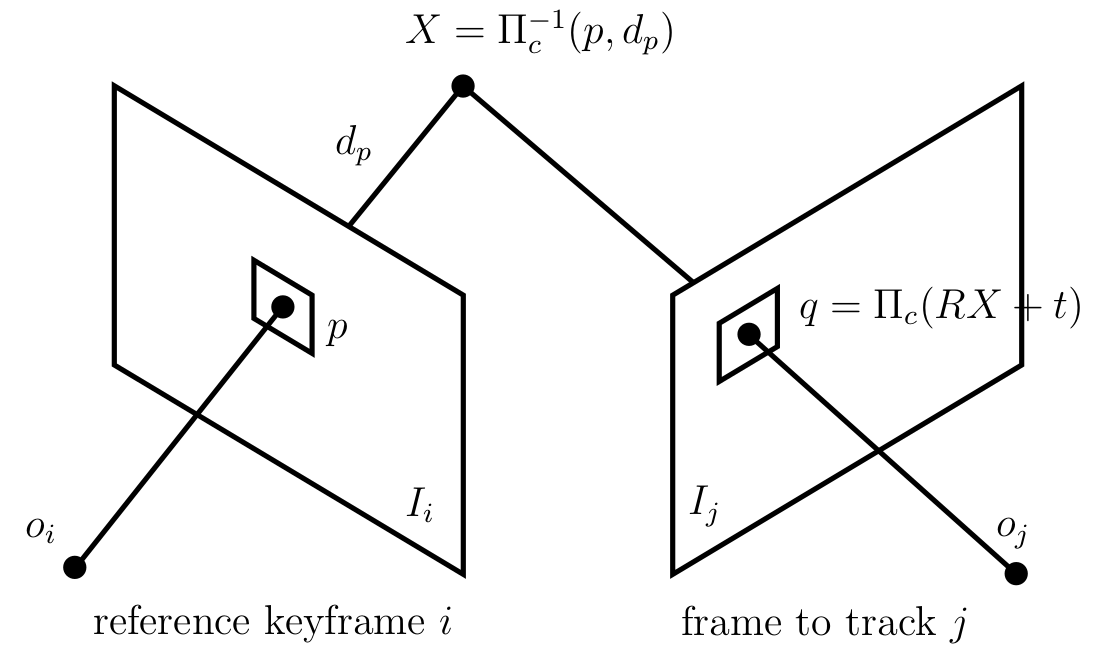
\includegraphics[width=\linewidth]{assets/img/direct-image-alignment.png}
	\caption{Direct image alignment}%
	\label{fig:direct-image-alignment}
\end{figure}

\begin{figure}[ht]
	\centering
	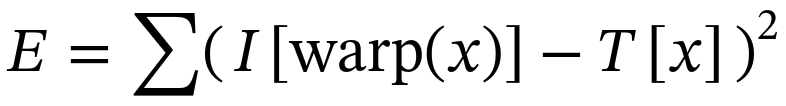
\includegraphics[width=\linewidth]{assets/img/energy-warp.png}
	\caption{Energy formulation for direct image alignment}%
	\label{fig:energy-warp}
\end{figure}

\begin{figure}[ht]
	\centering
	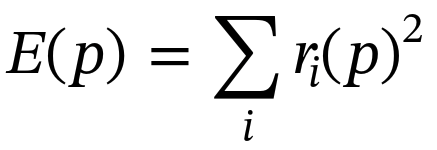
\includegraphics[width=\linewidth]{assets/img/energy-gauss-newton.png}
	\caption{Energy formulation for Gauss-Newton minimization}%
	\label{fig:energy-gauss-newton}
\end{figure}

\begin{figure}[ht]
	\centering
	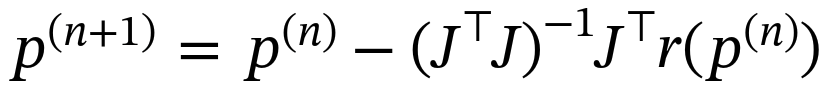
\includegraphics[width=\linewidth]{assets/img/gauss-newton-step.png}
	\caption{Gauss-Newton step}%
	\label{fig:gauss-newton-step}
\end{figure}

\subsection{RGB-D Visual Odometry}%
\label{sub:rgbd-visual-odometry}

\begin{figure}[ht]
	\centering
	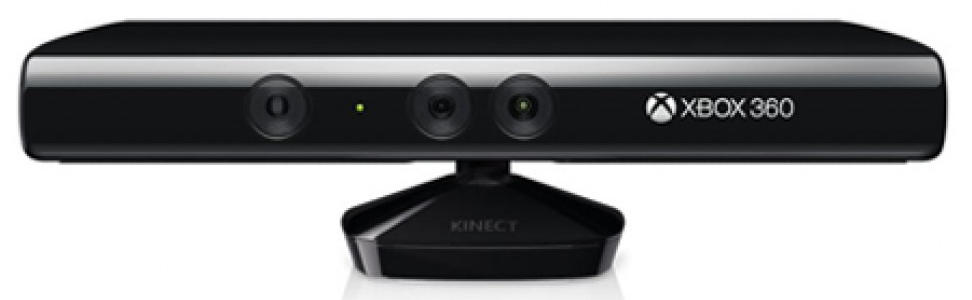
\includegraphics[width=\linewidth]{assets/img/kinect.jpg}
	\caption{Kinect sensor}%
	\label{fig:kinect}
\end{figure}

\section{Visual SLAM}%
\label{sec:v-slam}

\begin{figure}[ht]
	\centering
	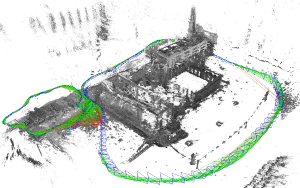
\includegraphics[width=\linewidth]{assets/img/lsd-slam.png}
	\caption{LSD-SLAM}%
	\label{fig:lsd-slam}
\end{figure}

\subsection{Pose Graph}%
\label{sub:pose-graph}

\begin{figure}[ht]
	\centering
	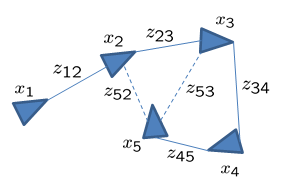
\includegraphics[width=\linewidth]{assets/img/pose-graph.png}
	\caption{Pose graph}%
	\label{fig:pose-graph}
\end{figure}

\subsection{Loop Closure}%
\label{sub:loop-closure}

\begin{figure}[ht]
	\centering
	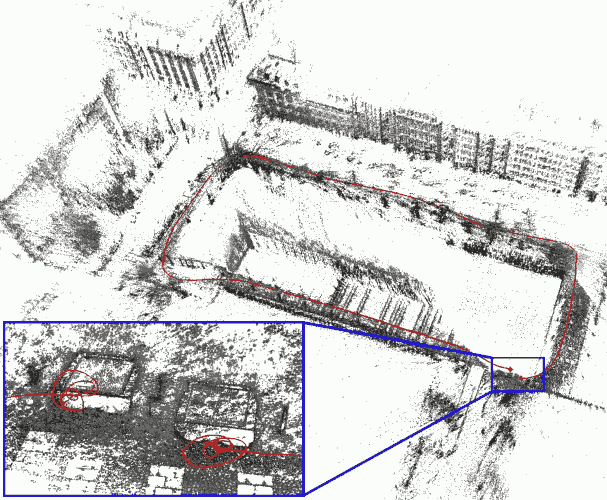
\includegraphics[width=\linewidth]{assets/img/loop-closure-lowres.png}
	\caption{Loop closure}%
	\label{fig:loop-closure}
\end{figure}
